%========== Compiler Directives ==========
% !TeX program = lualatex                                   
% !TeX encoding = utf8
% !TeX spellcheck = english

%========== Document settings ==========
\documentclass[11pt,a4paper,twoside,openany]{report}
\setlength\textwidth{145mm}
\setlength\textheight{247mm}
\setlength\oddsidemargin{14.2mm}
\setlength\evensidemargin{0mm}
\setlength\topmargin{0mm}
\setlength\headsep{0mm}
\setlength\headheight{0mm}
\let\openright=\cleardoublepage

%========== Language settings ==========
\usepackage[main=british,czech]{babel}

%========== Packages =============
\usepackage{thesis-package}

%========== Date format ===============
\newdateformat{monthyeardate}{\monthname[\THEMONTH] \THEYEAR}

%========== Bibliography ==========
\addbibresource{bibliography.bib}

%========== Draft settings ==========
\usepackage{lipsum}

\makeindex[intoc]
\makenomenclature
\renewcommand{\nomname}{Glossary of Symbols}
\begin{document}

    \pagenumbering{gobble}
    
    %========== Title page ==========
    % Suppress displaying the page number on the title page + count the following page as page 1 (not used)
    \begin{titlepage}
        % Define a new command for horizontal lines, change thickness here
\newcommand{\HRule}{\rule{\linewidth}{0.5mm}}
\center

%========== Header ==========
\textsc{\LARGE Czech Technical University in Prague,\\Faculty of Electrical Engineering}\\[1.5cm]
\textsc{\Large Master's thesis}\\[0.5cm]

%========== Title ==========
\HRule\\[0.6cm]
{\huge\bfseries Dual Circularly Polarized Waveguide Antenna}\\[0.3cm] % Title of your document
\HRule\\[1.5cm]

%========== Authors ==========
\begin{minipage}{0.45\textwidth}
    \begin{flushleft}
        \large
        \textit{Author}\\
        M. \textsc{Šimák}\\
        \textsc{Department of Electromagnetic Field}
    \end{flushleft}
\end{minipage}
~
\begin{minipage}{0.45\textwidth}
    \begin{flushright}
        \large
        \textit{Supervisor}\\
        doc. Ing. P. \textsc{Hazdra}, Ph.D.\\
        \textsc{Department of Electromagnetic Field}
    \end{flushright}
\end{minipage}

%========== Logo ==========
% Position at 3/4 of the screen
\vfill\vfill\vfill
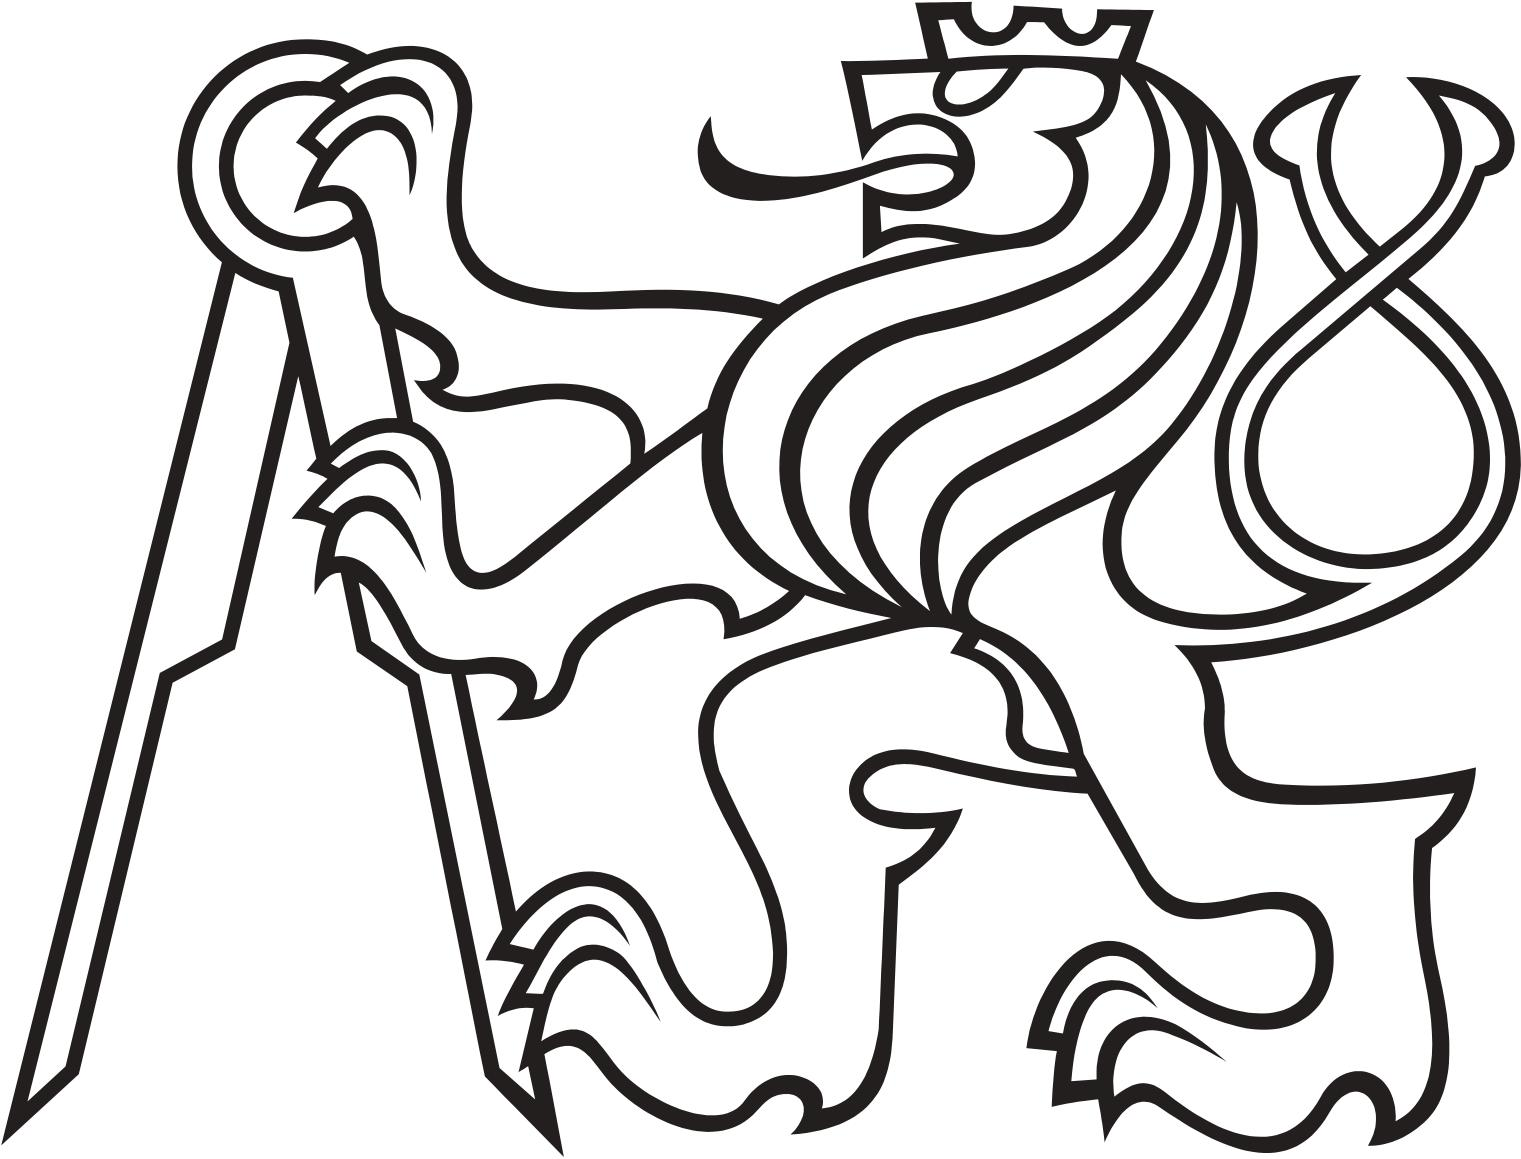
\includegraphics[width=0.3\textwidth]{src/ctu_logo_black.jpg}

%========== Date ==========
\vfill\vfill
{\large\monthyeardate\today}
% Push the date up 1/4 of the remaining page
\vfill
    \end{titlepage}

    %========== Blank page ==========
    \newpage\blankpage

    % %========== Assignment ==========
    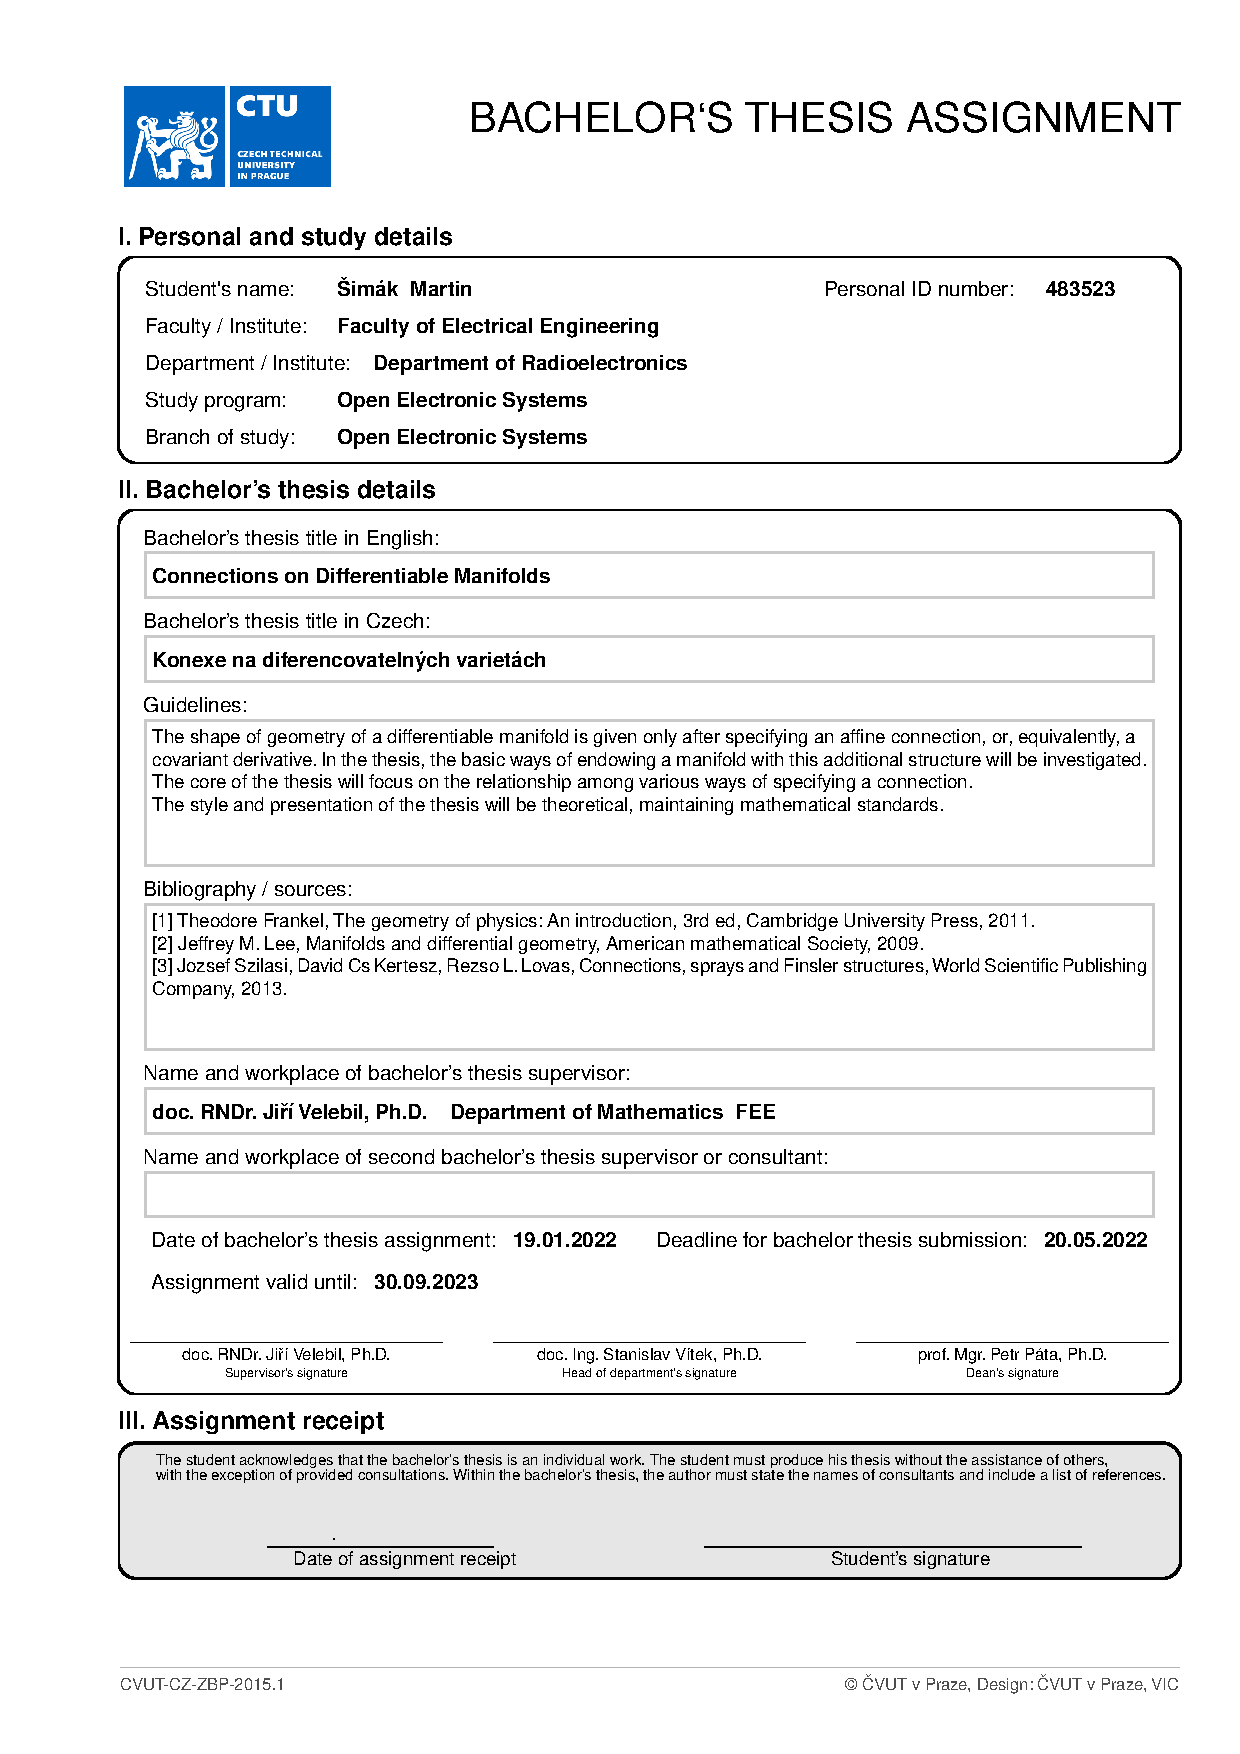
\includepdf[pages=-]{src/assignment.pdf}

    % Start counting pages in roman numerals
    \pagenumbering{roman}

    % %========== Declaration ==========
    % \clearpage
\vspace*{\fill}
\noindent\textbf{Declaration}\\[0.25cm]
I declare that I completed the presented thesis independently and that all used sources are quoted in accordance with the Methodological instructions that cover the ethical principles for writing an academic thesis.\\
\hrule\vspace*{1cm}
\begin{otherlanguage}{czech}
    \noindent\textbf{Prohlášení}\\[0.25cm]
    Prohlašuji, že jsem předloženou práci vypracoval samostatně a že jsem uvedl veškeré použité informační zdroje v souladu s Metodickým pokynem o dodržování etických principů při přípravě vysokoškolských závěrečných prací.\\
    \begin{center}
        \begin{minipage}{0.45\textwidth}
            \begin{flushleft}
                V Praze \hdashrule{3cm}{0.5pt}{2pt}
            \end{flushleft}
        \end{minipage}
        ~
        \begin{minipage}{0.45\textwidth}
            \begin{flushright}
                \noindent\begin{tabular}{c}
                    \\
                    \hdashrule{4cm}{0.5pt}{2pt}\\
                    Martin Šimák
                \end{tabular}
            \end{flushright}
        \end{minipage}
    \end{center}
\end{otherlanguage}
\clearpage

    % %========== Acknowledgements ==========
    % \clearpage
\vspace*{\fill}
\noindent\textbf{Acknowledgements}\\[0.25cm]
Above all, I would like to thank my supervisor, doc. Ing. Pavel Hazdra, Ph.D., for his professional help, willingness, and reliable correspondence throughout our collaboration, which took place remotely during my double degree program in cooperation with the National Taiwan University of Science and Technology. I would also like to thank my supervisor, Ding-Bing Lin, who is responsible for the content of this thesis at the partner university, for his initiative and valuable assistance, especially in the design production. Last but not least, I would like to thank all my loved ones who supported me from afar throughout my studies, especially my family and friends. Special thanks go to Ester \foreignlanguage{czech}{Jančaříková} for standing by me and helping me through difficult times.\\
\hrule\vspace*{1cm}
\begin{otherlanguage}{czech}
    \noindent\textbf{Poděkování}\\[0.25cm]
    Především bych rád poděkoval svému vedoucímu, doc. Ing. Pavlu Hazdrovi, Ph.D., za jeho odbornou pomoc, vstřícnost, a ochotu v podobě spolehlivé korespondence během spolupráce, která probíhala distančně v rámci mého studia double degree programu ve spolupráci s National Taiwan University of Science and Technology. Dále děkuji svému vedoucímu Ding-Bing Linovi, který odpovídá za náplň této práce na partnerské univerzitě, za jeho iniciativu a cennou pomoc, zejména při výrobě návrhu. V neposlední řadě bych rád poděkoval všem svým blízkým, kteří mě na dálku podporovali během celého studia, zejména své rodině a přátelům. Zvláštní poděkování na závěr potom patří Ester Jančaříkové za to, že stála při mě a byla mi oporou v nelehkých chvílích.
\end{otherlanguage}
\clearpage

    % %========== Abstract ==========
    % \clearpage
\noindent\textit{Title:}\\
\textbf{Dual Circularly Polarized Waveguide Antenna}\\[0.25cm]
\textit{Author:} Martin Šimák\\[0.25cm]
\textit{Study programme:} Electronics and Communications\\[0.25cm]
\textit{Supervisor:} doc. Ing. Pavel Hazdra, Ph.D., Department of Electromagnetic Field FEE\\[0.25cm]
\textit{Abstract:}\\
This thesis details the design, simulation, fabrication, and measurement of a novel dual circularly polarized antenna operating in the $\frequencyrange$ band. The system comprises a square waveguide polarizer with chamfered corners, a dual-coaxial feed, and a conical horn antenna. The polarizer generates right-hand and left-hand circular polarization by selectively exciting one of the two fundamental modes of the square waveguide. The dual coaxial feed provides the necessary excitation. The conical horn, designed using Antenna Magus and adapted to the polarizer, achieves a target gain of $\qty{15}{dBi}$. CST Studio Suite was used for electromagnetic simulations, while Python with SciPy enabled dynamic optimization for enforcing geometric constraints. The fabricated antenna's measured performance closely aligns with simulations, demonstrating an axial ratio below $\qty{5}{dB}$ across the band and a measured gain of approximately $\qty{18}{dBi}$ at the centre frequency. This work contributes to a compact, manufacturable, dual circularly polarized antenna design with potential applications in satellite communications, radar, and other wireless systems.\\[0.25cm]
\textit{Keywords:} circular polarization, waveguide polarizer, dual-feed, conical horn antenna, hexagonal waveguide, eigenmode analysis, electromagnetic simulation\\[0.5cm]
\begin{otherlanguage}{czech}
    \noindent\textit{Název práce:}\\
    \textbf{Duálně kruhově polarizovaná vlnovodová anténa}\\[0.25cm]
    \textit{Autor:} Martin Šimák\\[0.25cm]
    \textit{Studijní program:} Elektronika a komunikace\\[0.25cm]
    \textit{Vedoucí:} doc. Ing. Pavel Hazdra, Ph.D., Katedra elektromagnetického pole FEL\\[0.25cm]
    \textit{Abstrakt:}\\
    Tato diplomová práce popisuje návrh, simulaci, výrobu a měření duální kruhově polarizované antény pracující v pásmu $\frekvencnipasmo$. Systém se skládá ze čtvercového vlnovodného polarizátoru se zkosenými rohy, dvojitého koaxiálního napájení a kuželové antény. Polarizátor generuje pravotočivou a levotočivou kruhovou polarizaci selektivně buzené jedním ze dvou základních módů čtvercového vlnovodu. Potřebné buzení zajišťuje duální koaxiální napájení. Kuželová anténa navržená pomocí programu Antenna Magus a přizpůsobená polarizátoru dosahuje cílového zisku $\qty{15}{dBi}$. Pro elektromagnetické simulace byla použit software CST Studio Suite, zatímco Python s použitím knihovny SciPy umožnil dynamickou optimalizaci pro vynucení geometrických omezení. Naměřený výkon zhotovené antény se přesně shoduje se simulacemi a vykazuje osový poměr pod $\qty{5}{dBi}$ v celém pásmu a naměřený zisk přibližně $\qty{18}{dBi}$ na střední frekvenci. Tato práce přináší kompaktní, vyrobitelnou konstrukci duální kruhově polarizované antény s potenciálním využitím v satelitní komunikaci, radarové technice a dalších bezdrátových systémech.\\[0.25cm]
    \textit{Klíčová slova:} kruhová polarizace, vlnovodný polarizátor, duální napájení, kuželová anténa, hexagonální vlnovod, analýza vlastních módů, elektromagnetická simulace\\[0.5cm]
\end{otherlanguage}
\clearpage

    % Start counting pages in arabic numerals
    \pagenumbering{arabic}

    %========== Table of contents ==========
    \tableofcontents

    %========== Introduction ==========
    \chapter*{Introduction}
    \label{chap:introduction}
    \addcontentsline{toc}{chapter}{\nameref{chap:introduction}}
    
    Write a couple of words on literature survey. Present the difference construction and design choices, compare them both theoretically and by the results presented in gathered papers.
    \\
    \cite{rud-shpachenko:polarizers-on-sections-of-square-waveguides-with-inner-corner-ridges}
    \index{index entry}

    \lipsum[1-2]

    \paragraph*{Synopsis.} In \textbf{Chapter~\ref{chap:theory}}, \lipsum[3]

    \paragraph*{Methodology.} \lipsum[4]


    %========== Chapter 1: Theory of Operation ==========
    \chapter{Theory of operation}
    \label{chap:theory}

    \lipsum[5]

    Throughout the theory chapter, I will omit using the common \enquote{notation candy} of \emph{del}, or \emph{nabla}, for the vector differential operator $\nabla$ which gives rise to the formally proper differential operators of gradient ($\nabla$), divergence ($\nabla\cdot$), curl ($\nabla\times$), and sometimes even the Laplace operator ($\nabla\cdot\nabla$ or $\nabla^2$). Instead, I will use the standard notations of $\Grad$, $\Div$, $\Curl$, and $\Delta$, respectively. There are various reasons for this decision, e.g., that the definition of such an operator is inherently dependent on the working coordinate system, while the differential operators can be broadly extended beyond Cartesian or even Euclidean geometries, or that it promotes a notational ambiguity with the covariant derivative used in differential geometry. The main reason, however, is simply that the fundamental nature of the operator is undefinable and thus unclear.
    \nomenclature{$\Grad$}{gradient }%
    \nomenclature{$\Div$}{divergence }%
    \nomenclature{$\Curl$}{curl }%
    \nomenclature{$\Delta$}{Laplace operator }%

    Inspired by~\cite{balanis:advanced-engineering-electromagnetics}~and~\cite{griffiths:introduction-to-electrodynamics}.

    \section{Laws of electrodynamics}
    \label{sec:first-section}
        Lay out \texttt{the equations}, brr\\
        \begin{subequations}
            \label{eq:maxwell-general}
            \noindent\centering
            \begin{minipage}{0.45\textwidth}
                \begin{align}
                    \label{maxwell-general-div-d}
                    \Div\vec D &= \rho_{\mathrm e},
                \\
                    \label{maxwell-general-curl-e}
                    \Curl\vec E &= -\vec J_{\mathrm m} - \partial_t\vec B,
                \end{align}
            \end{minipage}
            \hfill
            \begin{minipage}{0.45\textwidth}
                \begin{align}
                    \label{maxwell-general-div-b}
                    \Div\vec B &= \rho_{\mathrm m},
                \\
                    \label{maxwell-general-curl-h}
                    \Curl\vec H &= \vec J_{\mathrm e} + \partial_t\vec D,
                \end{align}
            \end{minipage}
        \end{subequations}\\%
        % \nomenclature{$E$}{electric field intensity }%
        % \nomenclature{$B$}{magnetic field intensity }%
        % \nomenclature{$D$}{electric flux density }%
        % \nomenclature{$H$}{magnetic flux density }%
        % \nomenclature{$\rho_{\mathrm e}$}{electric charge density }%
        % \nomenclature{$\rho_{\mathrm m}$}{magnetic charge density }%
        % \nomenclature{$J_{\mathrm e}$}{source electric current density }%
        % \nomenclature{$J_{\mathrm m}$}{source magnetic current density }%
        \nomenclature{$\partial_\xi$}{partial derivative w.r.t. variable $\xi$ }
        \begin{itemize}
            \item $J_{\mathrm e}$ is total electric current made up of the source current $J_{\mathrm s}$ and conductive current $J_{\mathrm c}$. 
            \item $\rho_{\mathrm m}$ and $\vec J_{\mathrm m}$ are part of the \enquote{generalized} current concept.
            \item Explain the concept of these equations being expressed in \emph{free} charge and \emph{free} current. Give example of the Maxwell's equations neglecting the matter properties, to the convenience of which the \emph{free} sources are introduced, and make comments how equally general and useful they are.
            \item Comment on mathematical completeness together with boundary conditions which are usually \enquote{obvious}, such as vanishing potentials at infinity etc. Source Griffiths for that from his formulation without material properties. This might need the inclusion of Lorentz's force law for absolute completeness of electrodynamics.
        \end{itemize}
        
        \begin{align}
            \Div \vec J_{\mathrm{e}} &= -\partial_t\rho_{\mathrm{e}}
        \end{align}

        \subsection{Constitutive relations in time domain}
            \begin{subequations}
                \label{eq:constitutive-relations}
                \begin{align}
                    \label{eq:constitutive-relations-permittivity}
                    \vec D &= \hat\epsilon \ast \vec E,
                \\
                    \label{eq:constitutive-relations-permeability}
                    \vec B &= \hat\mu \ast \vec H,
                \\
                    \label{eq:constitutive-relations-conductivity}
                    \vec J_{\mathrm c} &= \hat\sigma \ast \vec E,
                \end{align}
            \end{subequations}
            % \nomenclature{$\hat\epsilon$}{permittivity }%
            % \nomenclature{$\hat\mu$}{permeability }%
            % \nomenclature{$\hat\sigma$}{conductivity }%
            where $\hat\epsilon$, $\hat\mu$, and $\hat\sigma$ are generally second rank tensors and $\ast$ denotes \emph{convolution}.
            
            \noindent%
            Talk about materials characterization
            \begin{enumerate}
                \item \emph{dielectrics}, \emph{magnetics}, and \emph{conductors}, with regard to their \emph{polarization}, \emph{magnetization}, and \emph{conduction};
                \item \emph{linear} versus \emph{nonlinear}, \emph{homogeneous} versus \emph{inhomogeneous}, \emph{isotropic} versus \emph{anisotropic}, and \emph{dispersive} versus \emph{nondispersive}. Mention the simplification of material tensors ($\ast\to\cdot$, $F(\vec r,t) \to F(t)$, matrix $\to$ scalar, $\partial_\omega = 0$).
            \end{enumerate}

            \noindent%
            In the simplest case of free space,~\eqref{eq:constitutive-relations-permittivity},~\eqref{eq:constitutive-relations-permeability},~and~\eqref{eq:constitutive-relations-conductivity} become
            \begin{align}
                \hat\epsilon &= \epsilon_0 \approx 8.854\times 10^{-12}\ \unit{F.m^{-1}},
            \\
                \hat\mu &= \mu_0 = 4\pi\times 10^{-7}\ \unit{H.m^{-1}},
            \\
                \hat\sigma &= 0\ \unit{S.m^{-1}}.
            \end{align}

        \subsection{Boundary conditions}
            Include if needed (probably will be).

        \subsection{Power and energy}
            Include Poynting theorem if needed.
    
        \subsection{Electromagnetic properties of matter}
            This one will, hopefully, be skippable. If not, talk about
            \begin{itemize}
                \item $\rho = \rho_{\mathrm f} + \rho_{\mathrm b} = \rho_{\mathrm f} - \Div\vec P$ due to free and bound charges,
                \item $\vec J_{\mathrm e} = \vec J_{\mathrm f} + \vec J_{\mathrm b} + \vec J_{\mathrm p} = \vec J_{\mathrm f} + \Curl \vec M + \partial_t\vec P$, where $\vec M$ is magnetic polarization (magnetization), due to free, bound and polarization currents,
            \end{itemize}
            from~\cite{griffiths:introduction-to-electrodynamics}.
    
    \section{Electromagnetic waves}
    \label{sec:electromagnetic-waves}
        
        \subsection{The wave equations}
            Inside regions with no \emph{free} charge or \emph{free} current,%
                \footnote{Expand on the notions of \emph{free} and \emph{bound} sources.}
            Maxwell's equations take the form of\\
            \begin{subequations}
                \label{eq:maxwell-sourceless}
                \noindent\centering
                \begin{minipage}{0.45\textwidth}
                    \begin{align}
                        \label{eq:maxwell-sourceless-div-d}
                        \Div \vec D &= 0,
                    \\
                        \label{eq:maxwell-sourceless-curl-e}
                        \Curl \vec E &= -\partial_t\vec B,
                    \end{align}
                \end{minipage}
                \hfill
                \begin{minipage}{0.45\textwidth}
                    \begin{align}
                        \label{eq:maxwell-sourceless-div-b}
                        \Div\vec B &= 0,
                    \\
                        \label{eq:maxwell-sourceless-curl-h}
                        \Curl\vec H &= \sigma\vec E + \partial_t\vec D.
                    \end{align}
                \end{minipage}\bigskip
            \end{subequations}\\
            Furthermore, if the medium is \emph{linear} and \emph{homogeneous}, equations \eqref{eq:maxwell-sourceless-curl-e}~and~\eqref{eq:maxwell-sourceless-curl-h} simplify to\\
            \begin{subequations}
                \label{eq:maxwell-sourceless-easy}
                \noindent\centering
                \begin{minipage}{0.45\textwidth}
                    \begin{align}
                        \label{eq:maxwell-sourceless-easy-div-e}
                        \Div \vec E &= 0,
                    \\
                        \label{eq:maxwell-sourceless-easy-curl-e}
                        \Curl \vec E &= -\partial_t\vec B,
                    \end{align}
                \end{minipage}
                \hfill
                \begin{minipage}{0.45\textwidth}
                    \begin{align}
                        \label{eq:maxwell-sourceless-easy-div-b}
                        \Div\vec B &= 0,
                    \\
                        \label{eq:maxwell-sourceless-easy-curl-b}
                        \Curl\vec B &= \mu\sigma\vec E + \mu\epsilon\partial_t\vec E.
                    \end{align}
                \end{minipage}\bigskip
            \end{subequations}

            Applying the curl to~\eqref{eq:maxwell-sourceless-easy-curl-e}~and~\eqref{eq:maxwell-sourceless-easy-curl-b} and using the identity $\Curl\Curl = \Grad\Div - \Delta$ from vector calculus, we obtain\\
            \begin{subequations}
                \label{eq:wave-equations}
                \noindent\centering
                \begin{minipage}{0.45\textwidth}
                    \begin{align}
                        \label{eq:wave-equation-e}
                        \Delta\vec E &= \mu\sigma\partial_t\vec E + \mu\epsilon\partial^2_t\vec E,
                    \end{align}
                \end{minipage}
                \hfill
                \begin{minipage}{0.45\textwidth}
                    \begin{align}
                        \label{eq:wave-equation-b}
                        \Delta\vec B &= \mu\sigma\partial_t\vec B + \mu\epsilon\partial^2_t\vec B.
                    \end{align}
                \end{minipage}\bigskip
            \end{subequations}\\
            Therefore electric and magnetic fields in linear homogeneous media both clearly satisfy the wave equation with a linear damping term $\mu\sigma\partial_t$ introduced by conductive losses. Furthermore, electromagnetic fields propagating in regions of zero conductive current, such as free space or ideal insulators, take the shape of the wave equations\\
            \begin{subequations}
                \label{eq:wave-equations-lossless}
                \noindent\centering
                \begin{minipage}{0.45\textwidth}
                    \begin{align}
                        \label{eq:wave-equation-e-lossless}
                        \Delta\vec E &= \mu\epsilon\partial^2_t\vec E,
                    \end{align}
                \end{minipage}
                \hfill
                \begin{minipage}{0.45\textwidth}
                    \begin{align}
                        \label{eq:wave-equations-b-lossless}
                        \Delta\vec B &= \mu\epsilon\partial^2_t\vec B,
                    \end{align}
                \end{minipage}\bigskip
            \end{subequations}\\
            which are ubiquitous in theoretical physics. Following the general notation, we can write\\
            \begin{subequations}
                \label{eq:wave-equations-lossless-dalembert}
                \noindent\centering
                \begin{minipage}{0.45\textwidth}
                    \begin{align}
                        \label{eq:wave-equation-e-lossless-dalembert}
                        \square\vec E &= 0,
                    \end{align}
                \end{minipage}
                \hfill
                \begin{minipage}{0.45\textwidth}
                    \begin{align}
                        \label{eq:wave-equations-b-lossless-dalembert}
                        \square\vec B &= 0,
                    \end{align}
                \end{minipage}\bigskip
            \end{subequations}\\
            where $\square = \Delta - 1/c^2\partial^2_t$ is the d'Alembert operator. Recognizing these as the wave equations hence immediately gives rise to the formula
            \begin{align}
                v &= \frac{1}{\sqrt{\epsilon\mu}} = \frac{c}{\sqrt{\epsilon_r\mu_r}}
            \end{align}
            for the speed of electromagnetic waves in linear homogeneous media.
            
            Compared with the original Maxwell's equations~\eqref{eq:maxwell-general}, these equations form two systems of partial differential equations of second order but are now decoupled and provide us with an additional solving method for given boundary-value problems. However, it is important to note that the wave equations~\eqref{eq:wave-equation-e}~and~\eqref{eq:wave-equation-b} were derived from Maxwell's equation by differentiation. This impedes their mathematical equivalence. More specifically (as stated in~\cite{griffiths:introduction-to-electrodynamics}), whereas every solution to Maxwell's equations is also a solution for the wave equations, the converse is not true.
        
        \subsection{Monochromatic plane waves}
            
            Maxwell's equations along with the constitutive relations all the theory outlined so far involves description of general vector fields which vary in space and time. However, we have shown in Section~\ref{sec:electromagnetic-waves}, the fields, given certain conditions, exhibit wave behaviour. Nonetheless, these fields still take the form of general vector fields which is far too complex for analysis in any practical systems. Luckily, many of these systems, such as just about any laboratory conditions can produce, the time variations of the produced fields are of harmonious nature. We may, therefore, confine our attention to \emph{time-harmonic} waves, also called \emph{monochromatic} waves,%
                \footnote{The etymology of this nomenclature comes from the Greek words \emph{m\'onos} (\enquote{sole, single}) and \emph{khr\^oma} (\enquote{color}).}
            of given frequency $\omega$.
            \begin{itemize}
                \item Chat about the possibility to express just about any function described as \enquote{wave} by a Fourier transform, consisting of such monochromatic waves, \url{https://en.wikipedia.org/wiki/Dirichlet%E2%80%93Jordan_test#Dirichlet_conditions_in_signal_processing}.
                \item Chat about plane waves travelling in the direction of wave vector $\vec k$ and find a way to introduce it.
                \item Finish the \emph{monochromatic} wave footnote.
            \end{itemize}
    
    %========== Conclusion ==========
    \chapter*{Conclusion}
    \label{chap:conclusion}
    \addcontentsline{toc}{chapter}{\nameref{chap:conclusion}}
    
    \lipsum[10-13]

    %========== Nomenclature ==========
    \printnomenclature
    
    %========== Bibliography ==========
    \printbibliography[heading=bibintoc]

    % %========== Index ==========
	\printindex

\end{document}
